% !TEX root = main.tex

\section{Overview}

Symbolic execution has been originally introduced in~\cite{K-CACM76} and~\cite{H-TSE77}. A good introduction to symbolic execution is presented in~\cite{KLEE-OSDI08}.\mynote{Extend this paragraph}
%(while~\cite{EXE-CCS06} is a previous effort of the same authors).
\cite{SAGE-NDSS08} is one successful story of symbolic execution. \cite{SAB-SP10} presents a neat formalization of symbolic execution and of taint analysis as well.

\subsection{Motivation}

Symbolic execution is a static analysis technique that has been introduced to perform automatic testing of
%complex
software. For instance, let us consider the C function shown in Figure~\ref{fig:example-1}. A critical operation performed in this code is the division on line 10. In principle, testing techniques such as random testing can generate bottomless input tests for this function, although it is unlikely that the inputs which make this code crash are effectively picked up by these techniques\mynote{Fuzzing?}. Indeed, albeit this code is relatively simple, too many assignments to the input values {\tt a}, {\tt b}, and {\tt c} are possible. Each {\tt int} input variable can be assigned to $2^{32}$ distinct values, but only those leading to $x + y + z - 3 = 0$ would make the code crash.

Symbolic execution overcomes common limitations of random testing techniques by evaluating a piece of code using {\em symbols} instead of concrete values for the inputs. The intuition behind it is to consider classes of input values instead of single instance values. Before analyzing how symbolic execution can identify the proper inputs which will make the function {\tt foobar} crash, we now introduce a few basic definitions.

\subsection{A Simple Execution Model}
\label{simple-execution-model}

Symbolic execution is a methodology for executing a program symbolically. In particular, every local or global variable is associated with a {\em symbol} of the form $\alpha_i$.  At any point of the execution, a symbolic engine has to maintain an execution state.

%\paragraph{Symbol} Any local or global variable is associated to a symbol $\alpha_i$. 
\paragraph{Execution state} An execution state $(stmt,~pc)$ is composed of two elements:
\begin{itemize}
  \item $stmt$: the statement to evaluate
  \item $pc$: a collection of path constraints, i.e., a set of assumptions made over the symbols $\alpha_i$ in order to reach $stmt$. Initially $pc$ is empty, and is thus trivially satisfied.
\end{itemize}

As in general every memory location can be associated with a symbol, an execution engine typically maintains also a {\em memory mapping} $M$ for storing constraints over different symbols.\mynote{Rephrase}

\paragraph{Execution model} In this section we discuss a simple language supporting assignments, conditional branches and jumps. A discussion of more complex constructs such as $call$, $return$, $while$, or $for$ will be provided in Section~\ref{example-discussion}. Depending on the kind of the statement $stmt$, the execution engine modifies the state as follows:
\begin{itemize}
  \item (constant assignment) $\alpha_i = c$: when a constant value $c$ is assigned to a variable associated to the symbol $\alpha_i$, $pc$ is extended by adding a constraint on $\alpha_i$:\mynote{Redundant?}
    \[ pc \gets pc \wedge \alpha_i = c\]
  \item (assignment) $\alpha_i = e$: when an expression $e$ is assigned to a symbol $\alpha_i$, $pc$ is extended by adding a constraint on $\alpha_i$:
    \[ pc \gets pc \wedge \alpha_i = e\]
  where $e$ can be any expression, involving unary or binary operators, over symbols and constants.
  \item (conditional branch) {\tt if} $e$ {\tt then} $s_{true}$ {\tt else} $s_{false}$: $pc$ is evaluated. Two scenarios are possible:
    \begin{itemize}
      \item (non-forking) $e$ is evaluated as always true or false under the assumptions in $pc$: the proper branch is taken, and symbolic execution advances to $s_{true}$ or $s_{false}$ accordingly;
      \item (forking) $e$ cannot be evaluated without instantiating values for one or more symbols in it: the symbolic execution process is forked, creating two execution states:
        \[ (s_{true}, pc_{true}) \text{ where } pc_{true} = pc \wedge e \]
        \[ (s_{false}, pc_{false}) \text{ where } pc_{false} = pc \wedge \neg e \]
    \end{itemize}
    Symbolic execution proceeds on both states in parallel.
  \item (jump) {\tt goto} $s$: execution state is updated to advance symbolic execution to $s$. 
  %\item (other constructs) A discussion of other constructs such as $call$, $return$, $while$, or $for$ is provided in Section~\ref{example-discussion}. 
\end{itemize}

\subsection{Example}
\label{symbolic-execution-example}

\begin{figure}[t]
\begin{lstlisting}[basicstyle=\ttfamily\small]
              1.  int foobar(int a, int b, int c) {
              2.    int x = 0, y = 0, z = 0;
              3.    if (a != 0)
              4.      x = -2;
              5.    if (b < 5) {
              6.      z = 2;
              7.      if (a == 0 && c != 0)
              8.        y = 1;
              9.    }
             10.    return a / (x + y + z - 3);
             11.  }
\end{lstlisting}
\label{fig:example-1}
\caption{Example: a very simple C function}
\end{figure}

\begin{figure}[t]
  \centering
  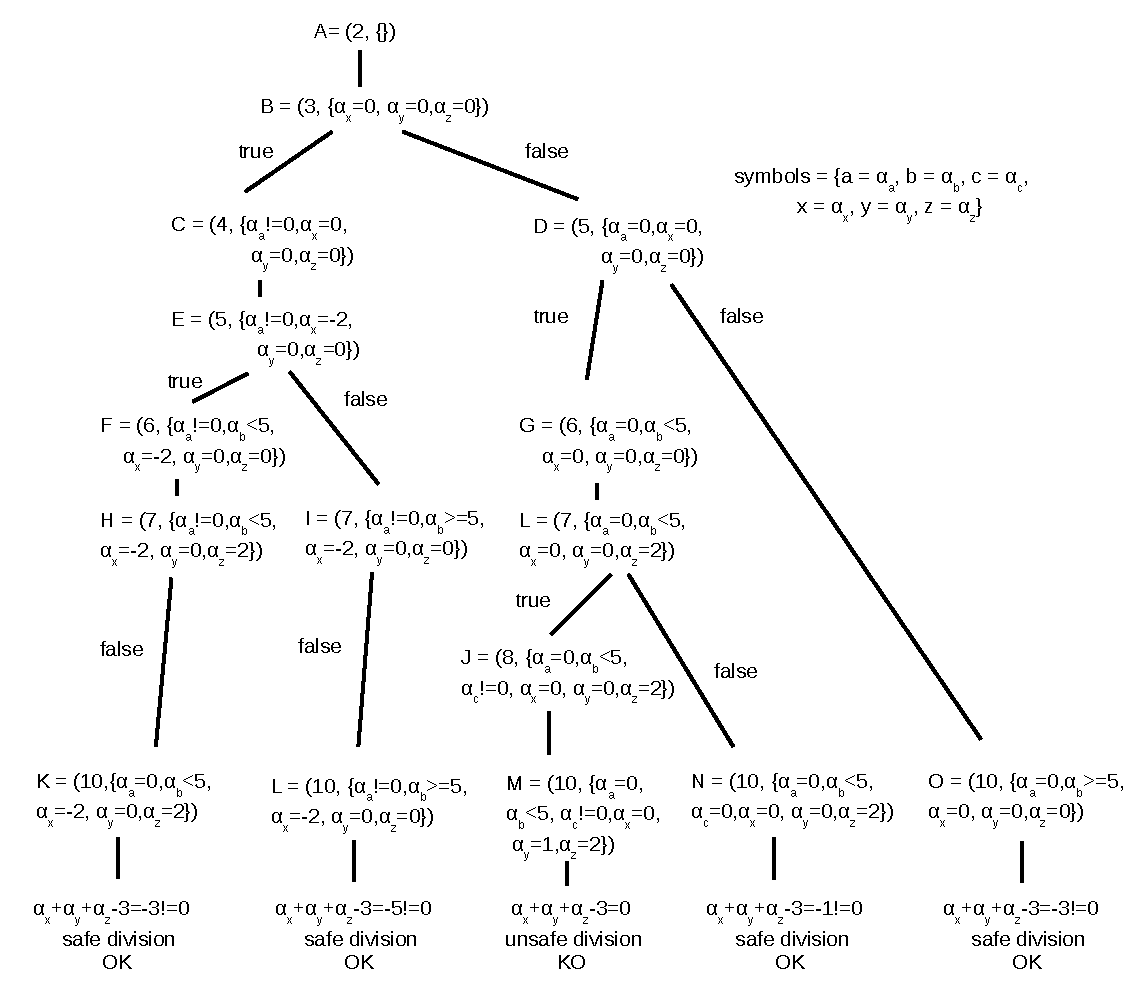
\includegraphics[width=1.0\columnwidth]{images/example} 
  \caption{Symbolic execution tree of the function {\tt foobar}. Each execution state is labeled with an alphabet letter. Side effects on execution states are highlighted in gray. Leaves are evaluated against division by zero error. For the sake of presentation the conjunction of constraints is shown as a list of constraints. }
  \label{fig:example-symbolic-execution}
\end{figure}

A symbolic execution of the function {\tt foobar} is shown in Figure~\ref{fig:example-symbolic-execution}. Initially, a new symbol is introduced for each input argument and for each local variable. For the sake of the presentation, we associate a symbol $\alpha_{var}$ with each variable $var$. 
Moreover, we assume that the set of local\mynote{locals only right? I added "at each point"} variables in use at each point by the function is known. In general, obtaining this information may be non trivial, and symbols are typically introduced when statements defining the variables are reached.
%Moreover, we have assumed to know the set of local variables used by the function. In general, obtaining this information may be non trivial and thus it it common to introduce symbols related to local variables only when the statements defining the variables are evaluated.
We also maintain a mapping table to track the mapping between variables and symbols. 

The first statement of the function is located at line 2. For this reason, the initial execution state $A$ is given by $(2, \{\})$ where the path constraint set is empty as no assumption is made on any symbol. After executing line 2,  $pc$ is updated by adding constraints on the value of $\alpha_x$, $\alpha_y$, and $\alpha_z$ (execution state $B$). Line 3 contains a conditional branch: since the condition cannot be uniquely determined based on the current set of assumptions, the execution is forked. Depending on the branch taken, a different statement is evaluated next and different assumptions are made on the symbol (execution states $C$ and $D$). On the other hand, when a condition can be uniquely determined (e.g., as in execution state $H$), it is sufficient to follow only the relevant branch (e.g., going to state $L$ from $H$), thus pruning unrealistic execution states. 

After expanding every execution state until the statement on line 10 is reached, we can check which input values for parameters {\tt a}, {\tt b}, and {\tt c} can make the function {\tt foobar} crash as a consequence of a division-by-zero operation. Analyzing execution states $\{L, M, N, O, P\}$, we can conclude that only $N$ can lead to an unsafe operation. The path constraint set for $N$ thus defines\mynote{implicitly defines?} the set of inputs that are unsafe for {\tt foobar}. Indeed, any input values for $\alpha_a$, $\alpha_b$, and $\alpha_c$ such that:
 \[ \alpha_a = 0 \wedge \alpha_b < 5 \wedge \alpha_c \neq 0 \]
will make the function crash. An instance of unsafe input parameters for {\tt foobar} can determined exploiting a constraint solver (i.e., an oracle able to resolve constraints). For instance, given the execution state $N$, a solver may come up with the values $a = 0$, $b = 1$, and $c = 0$. Notice\mynote{Say earlier?} that a constraint solver is also needed when evaluating the satisfiability of branch conditions.

\subsection{Discussion}
\label{example-discussion}

The example described in Section~\ref{symbolic-execution-example} shows the effectiveness of symbolic execution in identifying {\em all} the possible unsafe input values that can trigger a crash due to an unsafe division performed at line 10. This is achieved through an exhaustive exploration of all the possible execution states. For this reason, symbolic execution is a sound and complete methodology from a theoretical perspective. Soundness guarantees that input values deemed as unsafe are actually unsafe, and completeness implies that all possible unsafe inputs will be found. However, challenges that symbolic execution has to face when processing real-world code can be significantly more complex compared to those from our toy example of Figure~\ref{fig:example-1}. Several observations and questions naturally arise:

\begin{enumerate}

  \item (objects) {\em How does symbolic execution handle arrays or other more complex objects?} \\
  In general, any arbitrary complex object can be seen as an array of bytes, where each byte is associated with a distinct symbol. In principle, even a C {\tt int} variable can be seen as an array of four bytes.\mynote{Cosa intendiamo qui?} However, it is convenient to exploit structural properties of the data when possible (e.g., by statically analyzing the source code). For instance, for object-oriented languages the search performed by symbolic execution can be refined taking advantage of relational bounds on class fields.

  \item (loops) {\em How does symbolic execution handle loops?} \\
  In the execution model presented in Section~\ref{simple-execution-model} a loop can be encoded as a combination of conditional branches and $goto$ statements. This transformation is frequent when lowering a high-level language like C to an intermediate representation or native code. When the number of loop iterations cannot be determined in advance (e.g., it depends on an input parameter), for a symbolic execution engine choosing how many iterations should be analyzed becomes critical. The naive approach of unrolling iterations for every valid index bound leads to a very large number of states. It is possible to limit the number of iterations to $k$, thus trading speed for completeness, or when loop invariants can be inferred through static analysis they can be used to merge equivalent states (\mynote{Recuperare citazione}e.g., when differences are not observable outside the loop body).

  \item (subroutines) {\em How does symbolic execution handle subroutines?} \\
  Our execution model does not handle invocation of subroutines (i.e., a $call$ statement). \mynote{Extend this paragraph} A way to extend it to support subroutines is to provide the execution state with a simple execution stack.

  \item (recursion) {\em How does symbolic execution handle recursion?} \\
  Consider, as an example, the code:
    \begin{lstlisting}[basicstyle=\ttfamily\small]
    1.  int bar(int n) {
    2.    if (n >= 0) 
    3.      return 0;
    4.    return 1 + sum(n - 1);
    5.  }
    \end{lstlisting}
  Assuming that an execution stack has been added to the state, we observe that this code can easily lead to a very large number of execution states (i.e., a new state is subsequently created every time the branch on line 2 is not taken). As an {\tt int} variable can have up to  $2^{31} - 1$ positive values, symbolic execution has to create as many execution states to cover all the possible execution paths.
 %Indeed, the number of executions states is related to the number of times that the conditional branch on line 2 is not taken. 
 
  \item (environment) {\em How does symbolic execution handle interaction with the environment}? \\
  Real-world applications interacts constantly with the environment (e.g., filesystem, network) through libraries or system calls. A crucial aspect of these interactions is that they may cause side-effects
% on the environments 
(e.g., creation of a file)
%or initialization of a memory area
that must be taken into account, as they may later affect the 
%actual
execution of the code. Evaluating any possible outcome of an interaction is typically not feasible due to the large number of possibly generated execution states, only a small number of which can actually happen in a non-symbolic scenario. Hence, it is common to create models for popular library and system routines that help the symbolic execution engine to consider only significant outcomes.

  \item (state space explosion, path selection) {\em How does symbolic execution deal with path explosion}? \\
  A relatively simple code such as function {\tt foobar}, which is composed by less 12 lines of code, has generated 16 execution states, where $5$ out of $16$ are independent\mynote{Independent?} and must be checked to determine possible unsafe input values. Although this could seem a reasonable number of states, language constructs such as loops may contribute to increase the number of states exponentially. For this reason, it is unlikely that a symbolic execution engine is able to exhaustively explore all the possible execution states within a reasonable amount of time. In practice, heuristics are used to guide exploration and prioritize certain states first (e.g., to maximize code coverage), hoping this would lead to interesting discoveries. Also, a symbolic execution engine should implement efficient mechanism for evaluating multiple execution states in parallel without running out of resources.
  %In practice, several heuristics must be exploited to prioritize evaluation of some states, hoping to still be able to spot interesting things. Moreover, the symbolic execution engine should include efficient mechanism for efficiently evaluating in parallel different execution states without running out of computational resources.

  \item (constraint solver) {\em What can a constraint solver do in practice?}
  %{\em What is a constraint solver in practice}? \\
 Constraint solvers suffer from a number of limitations. Typically, they can handle complex constraints in a reasonable amount of time only if they are made of linear expressions over their constituents. Symbolic execution engines typically implement a number of optimizations to make queries as much {\em solver-friendly} as possible, for instance by splitting queries in independent components to process separately or by performing algebraic simplifications.

  \item (binary code) {\em What are the disadvantages of symbolically executing binary code}? \\
  The example presented in Section~\ref{symbolic-execution-example} is written in C. This does not imply that symbolic execution cannot be performed directly on binary code, which in several scenarios is the only available representation of a program. However, having the source code of an application makes symbolic execution significantly easier, as it can exploit high-level properties (e.g., object shapes) that can be inferred by statically analyzing the source code.
  %(e.g., the maximum size of a buffer or the number of iterations for a loop).
   
\end{enumerate}
%Depending on the specific application context of symbolic execution
Depending on the specific context in which symbolic execution is used, different choices and assumptions are made to address the questions highlighted above. Although they typically affect soundness or completeness, in several scenarios a partial exploration of the space of possible execution states is typically sufficient to reach the goal\mynote{Better example?} (e.g., identify a crashing input for an application) with a limited time budget.

%different choices and assumptions are made to address the above questions. Although soundness and completeness of symbolic execution may be negatively affected by these choices, there are several application scenarios where a partial exploration of the possible execution states is sufficient for reaching the ultimate goal (e.g., identify a single input that crashes an application).


%%%%%%%%%%%%%%%%%%%%%%%%%%%%%%%%%%%%%%%%%%%%%%%%%%%%%
\section{Memory model}
\label{memory-model}

A crucial aspect of symbolic execution is how the memory should be modeled. In other words, a symbolic engine may see symbols as distinct objects (i.e., each symbol is a distinct array of a specific size) or as pointers to a flat memory (i.e., index-based memory). Although the latter approach may seem more natural since it is akin to a concrete execution model, the former has been proved to be very effective in many scenarios since the symbolic constraints generated when using this approach are {\em easier} to parse for some solvers.

\subsection{Index-based memory}
\begin{itemize}
  \item memory is a map $\pi : I \to E$ from 32-bit indices ($i \in I$) to expressions ($e \in E$)
  \item load expressions $e = load(\pi, i)$: $i$ indixes $\pi$ and the loaded value $e$ represents the contents of the $i$-th memory cell
  \item store expressions $store(\pi, i, e)$: a new memory $\pi'$ where $i$ is mapped to $e$, i.e., $\pi' = \pi[i \gets e]$
\end{itemize}
When using this memory model, handling of arbitrary symbolic indices is notoriously hard, since a symbolic index may reference any cell in memory. Two approaches can be pursued: (a) concretization of the index where only a single value is evaluated for the index (see Section~\ref{concolic-execution} for more details), (b) fully symbolic memory where any possible value for the index is evaluated (e.g., \cite{BAP-CAV11}). The former is often excessively limiting (many paths are pruned away), while the latter is hard to make scalable. To overcome the limitations of both approaches, \cite{MAYHEM-SP12} models memory {\em partially}: symbolic writes are always concretized, while symbolic reads are allowed to be modeled symbolically.

\paragraph{Memory objects} Whenever there is a symbolic read, an immutable memory object $\mathcal{M}$ is generated:  it contains all values that could be accessed by the index, i.e., $\mathcal{M}$ is a partial snapshot of the global memory $\pi$. In practice, \cite{MAYHEM-SP12} reasons on $\mathcal{M}[i]$ instead of reasoning on $\pi[i]$, since the former is typically smaller than the latter.

\paragraph{Memory object bounds resolution} \cite{MAYHEM-SP12} trades accuracy with scalability by resolving the bounds $[\mathcal{L}, \mathcal{U}]$ of the memory region, where $\mathcal{L}$ is lower and $\mathcal{U}$ is the upper bound for the index $i$. Initially, $\mathcal{L} \in [0, 2^{32}-1]$. The solver is used to test if $i < \frac{2^{32}-1}{2}$ makes the path constrains unsatisfiable. If satisfiable then $\mathcal{L} \in [0, \frac{2^{32}-1}{2}]$, otherwise $\mathcal{L} \in [\frac{2^{32}-1}{2}, 2^{32}-1]$. The same strategy is repeated as much as possible. This is akin to a binary search algorithm. Whenever the bounds become reasonable, a memory object is generated. Unfortunately, there several cases where the bounds cannot be narrowed down drastically and thus other techniques can be used:
\begin{itemize}
  \item {\em value set analysis (VSA)}
  \item {\em refinement cache}
  \item {\em lemma cache}
  \item {\em index search trees (IST)}
  \item {\em bucketization with linear functions}
\end{itemize}
Whenever the size of the memory object exceeds a threshold (e.g., $|\mathcal{M}| \geq 1024$), then~\cite{MAYHEM-SP12} concretizes the index. However, instead of choosing a random value for the index, it tries to assign some {\em interesting} value (e.g., test it if it makes sense for it to be equal to an invalid memory address which can be exploited for security purposes).

\subsection{Object-based memory}

\cite{STP-TR07} is a decision procedure for bitvectors and arrays. Memory is seen as untyped bytes. Three data types are available:
\begin{itemize}
  \item {\em booleans}
  \item {\em bitvectors}: a fixed-length sequence of bits
  \item {\em arrays of bitvectors}
\end{itemize}
Most linear and non-linear operations are mapped to bitvector constraints. Conditional branches are transformaed into {\em multiplexers}, which are similar to C ternary operator. Bitvector operations are translated into operations to individual bits. Floating-points data types are not supported. Expresions types:
\begin{itemize}
  \item {\em formulas}, which have boolean values. They are converted into DAGs of single bit operations, where expressions with identical structure are represented uniquely (an hash table is maintain to track of existing expressions and lookups are performed on it when a new expression is created).
  \item {\em terms}, which have bitvectors values. They are converted into vectors of boolean formulas consisting entirely of single bit operations.
\end{itemize}

\paragraph{Mapping C code to STP primitives} Each C data block is represented symbolically as an array of 8-bit bitvectors. Typed operations in C generated constraints on the symbolic data (i.e., typeness is not actually known to~\cite{STP-TR07}). A mapping table is maintained to track symbolic data:
\begin{itemize}
  \item each input array $b$ is associated to a symbolic identically-size array $b_{sym}$ (i.e., the address of the C variable $b$ is mapped to the symbolic array $b_{sym}$ that is composed by $|b|$ 8-bit elements)
  \item $v = e$: an assignment expression, where $e$ is an expression that involves one or more symbolic data, adds a mapping between the address of $v$ and the generated symbolic expression $e_{sym}$. If $v$ is overwritten with a constant value or deallocated then this mapping is removed.
  \item $b[e]$: $b_{sym}$ is allocated, initializing it with the (constant) contents of $b$ (only if $b$ is actually initialized by a previous C statement). A mapping is added until $b$ is not deallocated.
\end{itemize}

\paragraph{Expression evaluation} An expression $e$ that contains some symbolic data can be seen as:
\[ l_1~~op_1~~l_2~~op_2~~l_3~~... \]
Each $l_i$ is evaluated in the following way:
\begin{itemize}
  \item if $l_i$ is concrete: the concrete value is used in the expression (e.g., if 4-byte $b$ is equal to 4 then the constant $000000...0100$ is used)
  \item otherwise: a concatenation of all the symbolic bytes of $l_i$ is used (e.g., $b_{sym}[0] @b_{sym}[1] @ $ $b_{sym}[2] @ b_{sym}[3] @ ...$)
\end{itemize}
Pointers are seen as array reference at some offset. This means that allocation sites as well as pointer arithmetic expressions must be instrumented in order to track where a pointer can point to. Notice that double dereferences ({\tt **p}) force~\cite{STP-TR07} to concretize the first dereference ({\tt *p}). 

\paragraph{Fast array transformations} Some transformations are needed to make\cite{STP-TR07} reason only on a purely functional language. In particular:
\begin{itemize}
  \item {\em read-over-write}: eliminates all write operations
    \[ read(write(A, i, v), j) \implies ite(i = j, v, read(A, j)) \]
    where $ite(a,b,c)$ is a ternary operator (i.e., if $a$ then $b$ else $c$). Notice that a write of a location without a subsequent read of the same location can be ignored.
  \item {\em read elimination}:
    \[ (read(A, i) = e_1) \wedge (read(A, j) = e_2) \]
    will be transformed in:
    \[ (v_1 = e_1) \wedge (v_2 = e_2) \wedge (i=j \implies v_1 = v_2) \]
  \item {\em array substitution optimization}
  \item {\em array-based refinement}
  \item {\em simplifications}: boolean or mathematical identities
\end{itemize} 

\paragraph{Optimizations} Other optimizations are applied:
\begin{itemize}
  \item {\em constraint caching}: cache solver results and reuse them
  \item {\em constraint independence}: tracks constraints into multiple independent subsets of constraints, This helps the system discards irrelevant constraints and adds additional cache hits.  
\end{itemize}

\section{Loops}

Loops can easily lead to the path explosion problem: any iteration of a loop can be seen as a {\tt IF-GOTO} statement. Example taken from~\cite{CS-CACM13}:
    \begin{lstlisting}[basicstyle=\ttfamily\small]
    1.  int N = sym_input(); // e.g., read
    2.  while (N > 0) {
    3.    N = sym_input();  
    4.  }
    \end{lstlisting}
The path constraint set of any final state will contain:
  \[ \left ( \bigwedge_{i \in [1, n]]} N_i > 0 \right ) \wedge (N_{n+1} \leq 0) \]
where $N_i$ is the symbol introduced at the i-th iteration.\\

For this reason, it is common to specifically deal with them:
\begin{itemize}

  \item {\em preconditions}: a technique to make it easier to perform symbolic execution on loops is through imposing some preconditions, e.g., use static analysis techniques to understand number of iterations for a loop. See Section~\ref{precontioned-symbolic-execution} for more details.

  \item {\em fixed exploration}: depending on the goal, a symbolic engine may decide to fully explore a loop (e.g., see heuristics presented in~\cite{AEG-NDSS11} and discussed in Section~\ref{heuristics}) or explore only a fixed number of iterations (e.g., up to 3 iterations) in order to avoid path explosion.

  \item {\em approximations}: effects of a loop are often approximated using {\em fixpoints} (e.g., in~\cite{KKM-USEC05,BNS-SP06,CFB-ACSAC06}). A fixpoint F is an approximation of the effect of loop body on an execution state. F approximates the state after the execution of loop whenever the initial state before the loop was F (?). Transforming an execution state to a fixpoint state is defined as widening. Construction of the fixpoint:
  \begin{itemize}
    \item S1: state after first iteration
    \item S2: state after second iteration
    \item compare S1 and S2: assign bottom to each symbol that has been altered
    \item repeat until there is no difference between Si and Si+1
    \item if there is a branch inside the loop, then either the branch is known or its condition is on a symbol which has been assign to bottom. In this case, two parallel states are created and then compared.
  \end{itemize}

\end{itemize}

Notice that detection/analysis of loops can be done using techniques such as~\cite{SGL-TOPLAS96} (e.g., in~\cite{CFB-ACSAC06}).

\section{Subroutines and recursion}

\section{Interaction with environment}

Environment can be seen as an input source. Since it can be unfeasible to analyze all possible interactions with the environment, it is common to model these interactions, emulating their behaviors and their side-effects. The main intuition is that models understand the semantics of the desired actions well enough to generate the required constraints.\\

\cite{KLEE-OSDI08}:
\begin{itemize}
  \item {\em file system}: operations on concrete files are actually performed. Operations on symbolic files are emulated modeling a simple symbolic file system, which is private for each execution state. Symbolic file system is a directory with $N$ symbolic files. Users specify both the number of files and their sizes. Any operation on a unconstrained symbolic file will generate $N+1$ branches: one for each symbolic file, plus one for a failing scenario. Emulation done at library level, not system call level. This make symbolic execution simpler (no need to symbolically execute library code) but assumption that library code is correct. If needed, library code is tested separately.
  \item {\em environment failures}: \cite{KLEE-OSDI08} emulates failures (e.g., failures of {\tt write}). This is optional since some applications may be not sensitive to environment failure.
  \item {\em re-running test cases}: inputs which may crash an application may depend on the environment failures. To force concrete execution towards failures, \cite{KLEE-OSDI08} exploits {\tt ptrace}.
\end{itemize}

\cite{AEG-NDSS11}:
\begin{itemize}
  \item {\em symbolic files}: emulation of {\tt open}, {\tt read}, {\tt write}, and similar other system calls. Similar to~\cite{KLEE-OSDI08}.
  \item {\em symbolic sockets}: emulation of {\tt socket}, {\tt bind}, {\tt accept}, {\tt send}, and similar other system calls. 
  \item {\em environment variables}: a complete summary of all possible results (concrete values, fully symbolic, and failures) of {\tt get\_env}.
  \item {\em library function calls and system calls}: emulation of more than 70 library routines and system calls. In particular, formatting functions (e.g., {\tt fprintf}) are emulated to capture buffer overflows.
\end{itemize}

\cite{DART-PLDI05}: external interfaces are extracted by analyzing library and system calls, then random results are returned (compliant with the type).

\section{State space explosion}

The main challenge with symbolic execution is managing the state space explosion problem. Since symbolic execution forks off a new interpreter at every (undecidable) branch, the total number of interpreters is exponentially in the number of of branches.

\subsection{Preconditioned symbolic execution}
\label{precontioned-symbolic-execution}

\cite{AEG-NDSS11} has proposed {\em preconditional symbolic execution} as a novel method to target symbolic execution towards certain subset of the input state space. The state space subset is determined by the precondition predicate $\Pi_{prec}$: inputs that do not satisfy $\Pi_{prec}$ will not be explored. The intuition for preconditioned symbolic execution is that we can narrow down the state space we are exploring by specifying exploitability conditions as a precondition, e.g., all symbolic inputs should have the maximum size to trigger buffer overflow bugs. The main benefit from preconditioned symbolic execution is simple: by limiting the size of the input state space before symbolic execution begins, we can prune program paths and therefore explore the target program more efficiently.
Note that preconditions cannot be selected at random. If a precondition is too specific, we will detect no bugs or exploits; if it is too general, we will have to explore almost the entire state space. %Thus, preconditions have to describe common characteristics among exploits (to capture as many as possible) and at the same time it should eliminate a significant portion of non-exploitable inputs.\\

Preconditioned symbolic execution enforces the precondition by adding the precondition constraints to the path predicate during initialization. Adding constraints may seem strange since there are more checks to perform at branch points during symbolic execution. However, the shrinking of the state space -- imposed by the precondition constraints -- outweighs the decision procedure overhead at branching points. When the precondition for a branch is unsatisfiable, we do no further checks and do not fork off an interpreter at all for the branch.% We note that while we focus only on exploitable paths, the overall technique is more generally applicable.\\

\paragraph{Preconditions} Kinds of preconditions:
\begin{itemize}
  \item {\em None}. There is no precondition and the state space is explored as normal.
  \item {\em Known Length}. The precondition is that inputs are of known maximum length. Static analysis techniques can be used to automatically determine this precondition.
  \item {\em Known Prefix}. The precondition is that the symbolic inputs have a known prefix.
  \item {\em Concolic Execution}. Concolic execution [24] can be viewed as a specific form of preconditioned symbolic execution where the precondition is specified by a single program path as realized by an example input. For example, we may already have an input that crashes the program, and we use it as a precondition to determine if the executed path is exploitable. See Section~\ref{concolic-execution} for a more detailed discussion of this technique.
\end{itemize}

\paragraph{An example} Consider the example:

\begin{lstlisting}[basicstyle=\ttfamily\small]
    // N symbolic branches 
    if (input[0] < 42) [...]
    [...]
    if (input[N - 1] < 42) [...]

    // symbolic loop
    strcpy(dest, input); 

    // M symbolic branches
    if (input[N + 1] < 42) [...]
    [...]
    if (input[N + M - 1] < 42) [...]
    \end{lstlisting}
where {\tt input} is an array of {\tt S} bytes. Impact of preconditions:
\begin{itemize}
  \item {\em None}. No constraint is added. State space is $2^N \cdot S \cdot 2^M$.
  \item {\em Known Length}. For instance, we add constraint that $(S - 1)$ bytes of {\tt input} are not equal to \textbackslash0. Since the symbolic loop is known, then the state space is reduce to $2^N \cdot 2^M$.
  \item {\em Known Prefix}. For instance, we add constraint that the $P$ bytes of {\tt input} are known ($P < N < S$). E.g., fixed header string). Since first $P$ branches and first $P$ iterations are concrete, then state space is $S \cdot 2^{N-P} \cdot 2^M$.
  \item {\em Concolic Execution}. We decide the exact values for all bytes of {\tt input}. Input space is $1$.
\end{itemize}

\subsection{Dynamic symbolic execution}


\paragraph{Concolic execution}
\label{concolic-execution}
{\em Concolic execution} has been originally introduced in~\cite{DART-PLDI05} and then refined by~\cite{CUTE-FSE13}. A common disadvantage of symbolic execution is that the state space can be exponential. Moreover, even when the state space is tractable it may happen that complex constraints need to be solved but these constraints are too complex for the actual solver (e.g., non-linear constraints are typically hard to solve). For this reason, it is common to exploit concolic execution. Different scenarios:
\begin{itemize}
  \item {\em Use concolic execution to generate useful (random) inputs.} Starts concrete execution using a random (concrete) input and for each taken branch tracks the input constraints by observing the branch condition. When the execution is completed, restart another concrete execution using a different concrete random input that is compliant with the constraints but explore a new path. It is sufficient to negate a single constraint given by a conditional branch, to explore a different path. Keep track of taken branches with binary values. An algorithm for maximizing coverage is proposed in~\cite{DART-PLDI05}. Notice that the symbolic execution is performed in parallel with the concrete execution. Related examples are~\cite{SAGE-NDSS08,DRILLER-NDSS16}. In particular,~\cite{DRILLER-NDSS16} is an example of {\em symbolic-assisted fuzzing}: their technique temporarily exploits concolic execution only when a fuzzer cannot generate a valid input to explore an uncovered branch.

  \item {\em Use concolic execution to overcome unsolvable constraints}. Assume to start a concrete execution with a concrete input and in parallel symbolically execute the same program. Whenever a set of constraints cannot be solved by the constraint solver, then use the concrete value to proceed into at least one branch. Example taken from~\cite{CS-CACM13}:
    \begin{lstlisting}[basicstyle=\ttfamily\small]
    int non_linear(int v) {
      return (v * v) % 50;
    }
    \end{lstlisting}
  The non-linear operation inside this function can be hard for a solver. Using a concrete execution, the engine can overcome this problem, but then the precision and completeness may be affected.

  Notice that the use of concrete values can also avoid to perform alias analysis on pointers, which is typically very expensive. Whenever meaningful, \cite{DART-PLDI05} tries to test both valid (not {\tt NULL}) and invalid ({\tt NULL}) input pointers in order to maximize bug detection. However~\cite{DART-PLDI05} will never artificially negate a branch if that condition cannot be exercised using a concrete input. In other words, both branches of an {\tt if} statement are considered only if they are both meaningful (more precisely: \cite{DART-PLDI05} is able to generate a valid input). Notice that~\cite{DART-PLDI05} may generate an input using a solver by considering only a subset of branch constraints. For instance, consider constraints ($C_1, C_2, C_3$) given by three nested branches: if $C_1$ is non linear (hard to solve), it needs only to generate a random input for taking $C_1$ and then use the solver for exploring path given by $(C_2, C_3)$. A traditional symbolic execution engine may get stuck at $C_1$ and give up after some time on {\em all} the derived path. Notice that whenever a concrete input is used to overcome a hard constraint, the overall approach become incomplete.

\end{itemize} 



Errors related to concrete values and 
\paragraph{Execution-Generated Testing} {\em Execution-Generated Testing (EGT)} is the approach used by some papers (e.g.,~\cite{KLEE-OSDI08,EXE-CCS06}) that works by making a distinction between the concrete and symbolic state of a program: if an operation involves only concrete values, then the symbolic engine concretely execute it. This can allow symbolic execution to reason even over complex operation (e.g., non linear operations) if they involve only concrete values. EGT is often seen (\cite{CS-CACM13}) as a form of dynamic symbolic execution: this can be seen as more general term than concolic execution.

\subsection{Under-constrained symbolic execution} 

By isolating a function from the rest of the program, we can perform symbolic execution on it. The results from this analysis can be exploited when any other program is symbolically executed and a call to the function is present. However, detected errors in the isolated function may be false positives since some of the input values may never been valid when the function is actually executed in the context of the full program. {\em Under-constrained symbolic execution}~\cite{ED-ISSTA07} is a technique that performs symbolic execution of an isolated function but clearly marks which symbols are {\em under-constrained} to distinguish them from the {\em exactly-constrained} symbols.

Errors due to concrete values and exactly-constrained symbols are treated as true positives. Errors due to under-constrained are treated as true positives only if {\em all} solutions to the currently known constraints on the symbols cause the error to occur. Otherwise the negation of the error is added to the constraint set and the symbolic execution of the isolated function is continued. In other words, an error is reported if and only if it is {\em context-insensitive}. Notice that a symbol may initially be under-constrained and then become exactly constrained. For instance, consider the following piece of code:
    \begin{lstlisting}[basicstyle=\ttfamily\small]
    assert(a != 0); // no knowledge about this variable
    a = 0;          // from now on we know the value of a
    assert(a != 0); // we always hit this error: context-insensitive! 
    \end{lstlisting}
The first {\tt assert} will not trigger an error: indeed, there is at least one possible value for the symbol associated to {\tt a} that does not hit the error. Conversely, the second {\tt assert} will always trigger an error since {\tt a} has a concrete value and it's not under-constrained anymore.\\

Although this technique is not able to find {\em all} the possible errors in a function, it still can find interesting bugs. Moreover, since symbolically executing a full program may be unfeasible, this technique can make it feasible to test tons of line of code in a reasonable amount of time. In particular, this technique allows an engine to skip code: if a function or any other construct (e.g., a loop) may be troublesome for symbolic execution, it can be skipped by just marking the locations affected by it as under-constrained. However, a possible implementation issue is given by the propagation of under-constrained symbols: given the line of code {\tt if (s < t)}, if {\tt t} is under-constrained while {\tt s} is exactly constrained then when the symbolic execution is proceeded into the two possible branches, {\tt s} must be marked as under-constrained. Some optimization may be needed in order to minimize this propagation effect.

\paragraph{Under-constrained KLEE} In~\cite{UCKLEE-USEC15}, KLEE~\cite{KLEE-OSDI08} has been extended in order to support under-constrained symbolic execution . In particular, these are some of the main improvements:
\begin{itemize}
  \item {\em Lazy initialization.} Whenever there is a pointer that is not concrete and without any active constraint (i.e., it is unbound), it its value is checked against {\tt NULL} then two path are analyzed: (a) where the pointer is {\tt NULL} and (b) where the pointer is pointing to a freshly allocated block of memory, whose content is marked as unbound.This means that pointer aliasing is assumed to not occur. In both paths, the pointer is not longer unbound.  In path (b), any test against the pointer is known and dereferences will be successfully resolved. Lazy initialization is common for data structure and thus it is common to bound its maximum length (i.e., {\em k-bounding}) in order to prevent the engine from allocating an unbounded number of objects.
  \item {\em Patch checking.} The main goal of~\cite{UCKLEE-USEC15} is to detect if a patch has introduced new bugs. In order to do so, it symbolically executes two compiled versions of a function: $P$, the unpatched version, and $P'$, the patched version. If it finds any execution paths along which $P'$ crashes but $P$ does not (when given the same symbolic inputs), it reports a potential bug. Indeed, due to missing input preconditions, not all crashes are real bugs: if both $P$ and $P'$ crash on an input, then maybe the crash is given by the unknown preconditions. 
  \item {\em Pruning techniques.} Using a static cross-checker (that navigates the control-flow graph and marks differing basic block between $P$ and $P'$), \cite{UCKLEE-USEC15} prunes paths that have never executed a differing basic block and that cannot reach a differing basic block from their current program counter and call stack. Moreover, $P'$ is executed before executing $P$, allowing the system to prune paths that return from $P'$ without triggering an error, or that trigger an error without reaching different blocks.
  \item {Dealing with false positives.} Two approaches are pursued to limit false positives:
    \begin{itemize}
      \item {\em manual annotations}: examples are data types invariants or preconditions upon function calls.
      \item {\em automated heuristics}: {\em must-fail} heuristics identify errors that must occur for all input values following that execution path. For instance, {\em belief-fail} heuristic checks if a function contradicts itself (e.g., a code checks that a pointer is {\tt NULL} and then dereferences it). Another variation of must-fail heuristic is {\em concrete-fail} that an assertion failure or memory errors was triggered by a concrete condition or pointer.
    \end{itemize}
  \item {\em Rule-based checkers.} Several rule-based checkers have been built on top of UCKLEE. They do a similar job such as other dynamic tools (e.g., {\em memcheck} for memory leaks and uninitialized data) but reasoning on all possible paths, not just the concrete ones. Moreover, user inputs can be considered as fully constrained (i.e., no assumption is valid on it since the code should sanitize it). 
  \item {\em Optimizations.} Some optimizations:
    \begin{itemize}
      \item Symbolic objects have a symbolic size: whenever there is an access to the object content, the system verifies if the offset could exceed the object's symbolic size. whenever path is considered where the offset does not exceed the symbolic size, then a lower bound on the symbolic size is set.
      \item Some library functions (e.g., {\tt strlen}) have been replaced with variants that do not lead to path explosion
      \item Scores of rules to simplify symbolic expressions
      \item {\em lazy constraints}: defer evaluation of constraints using a solver as much as possible. For instance, if there is an hard constraint on branch, take both branches and if an error is found check if that branch was actually valid.
      \item function pointers should be made concrete by the user.
    \end{itemize}

\end{itemize}


\subsection{State merging}

Several static program analysis techniques such as abstract interpretation merge states corresponding to different paths into a state that over-approximates them. In a precise symbolic execution, however, merging is not allowed to introduce any approximation or abstraction, and therefore can only change formulas to have them characterize sets of execution paths. In other words, a merged state will be described by a formula that represents the disjunction of the formulas that would described the individual states if they were kept separate.

\paragraph{An example} Let's consider the following piece of code (taken from~\cite{VERITESTING-ICSE14}):\mynote{customize example and improve discussion}
    \begin{lstlisting}[basicstyle=\ttfamily\small]
    B1: if (x > 1) 
    B2:   y = 42;
    B3: else if (x < 42) 
    B4:    y = 17;
    B5: else ;
    B6: ;
    \end{lstlisting}
Then a symbolic execution engine may perform state merging in the following way:
\begin{figure}[H]
  \centering
  \vspace{-3mm}
  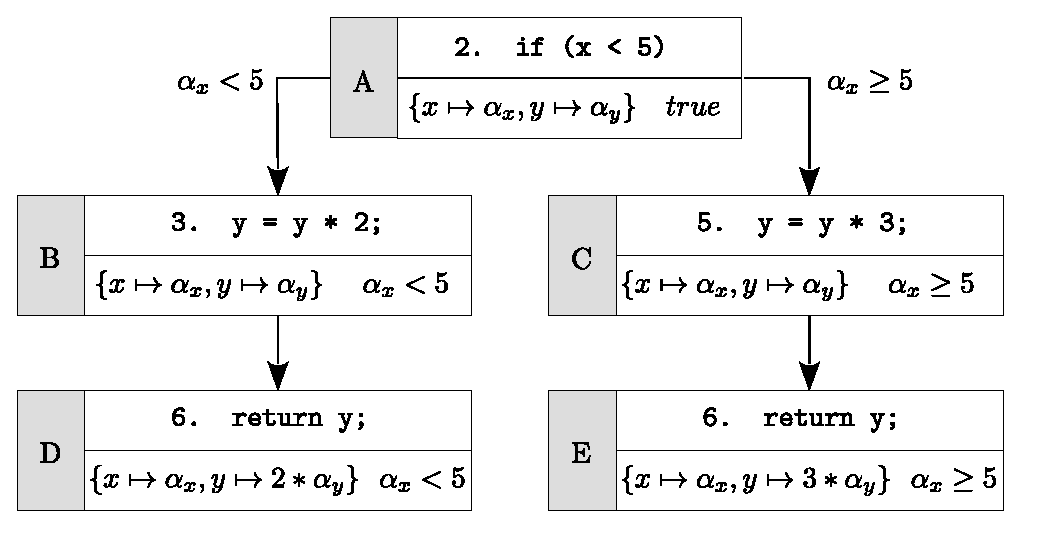
\includegraphics[width=0.65\columnwidth]{images/state-merging} 
  \vspace{-3mm}
  %\label{fig:example-symbolic-execution}
\end{figure}
where {\em ite} statements represents {\tt if-then-else} statements and $\bot$ stands for a non-taken branch.

\paragraph{Trade-off} Early work~\cite{G-POPL07,HSS-RV09} has shown that merging techniques effectively decrease the number of paths to explore, but also put a burden on constraints solvers, which typically encounter difficulties when dealing with disjunction. Merging can also introduce new symbolic expressions in the code, for instance when merging different concrete values from a conditional assignment into a symbolic expression over the condition. \cite{KKB-PLDI12} provides an excellent discussion of the design space of state merging techniques. At one end of the spectrum, search-based symbolic execution (as implemented, e.g., in~\cite{KLEE-OSDI08}) does not perform any merge. The other extreme is complete static state merging, implemented by verification condition generators, e.g, ~\cite{SATURN-POPL05,CALYSTO-ICSE08}), that combines states at join points after all the subpaths have been encoded.

\mynote{Function summaries}

\paragraph{Selective state merging} Intermediate merging solutions can adopt heuristics for driving both merging decisions and CFG exploration. Generating larger symbolic expressions and possibly extra solvers invocations can outweigh the benefit of having fewer states, leading to poorer overall performance~\cite{HSS-RV09,KKB-PLDI12}. Moreover, in order to maximize the opportunities for merging a symbolic execution engine should traverse the CFG in a topological order, which denies search exploration strategies aiming at prioritizing more ``interesting'' states over others.

Recent works (e.g., \cite{KKB-PLDI12} and \cite{VERITESTING-ICSE14}) have introduced novel techniques to tackle these issues: 
\begin{itemize}

  \item {\em query count estimation} identifies state merges that can reduce exploration time. This technique relies on a simple form of static analysis to identify how often each variable is used in branch conditions past any given point in the CFG. The estimate is used as a proxy for the number of solver queries that a given variable is likely to be part of. When two states are sufficiently similar, the overhead from solving more complex queries is likely to be outweighed by the savings from exploring fewer paths.

  \item {\em dynamic state merging} efficiently combines static state merging with common search heuristics. This technique allows merging of states that do not share the same program location. This is useful, for instance, for unbounded loops for which search-based symbolic execution engines would employ search strategies that prioritize exploring new code over unrolling, while static state merging would require a depth-first exploration and thus fully unroll the possibly infinitely many iterations of the loop. Dynamic state merging can consider for merging states that are likely to become similar in a small number of execution steps: this is likely to happen if one state is similar to one of the predecessors of the other. The intuition behind the algorithm is that if two states are similar, then also their two respective successors are likely to be similar after a few steps.

  \item {\em veritesting} dynamically identifies set of statements that generate formulas which are easy for solvers. Using a dynamically recovered CFG, it detects pieces of code that do not contain system calls, indirect jumps, or other statements that are difficult to precisely reason about statically. In particular, frontiers of hard-to-analyze statements are identified. Easy to analyze set of statements are then analyzed maintaining a single formula that describe all the merged states, while hard to analyze set of statements are evaluated using separate states pursuing the traditional symbolic execution approach.

\end{itemize}

\subsection{Limiting state space through other program analysis techniques}

Other static or dynamic techniques can be used to help a symbolic engine to focus on interesting states:
\begin{itemize}
  \item {\em program slicing}
  \item {\em taint-analysis}
  \item {\em source code analysis}: extraction of input properties (e.g., size or contents of an array)
  \item {\em phi-node folding transformation}: add select operations to merge statically paths (see, e.g., \cite{CCK-EUROSYS11})
  \item {\em compositional techniques}: caching and reusing the analysis of lower-level function in subsequent computations. The main idea is to compute function summaries. See, e.g.,~\cite{G-POPL07,G-PLDI11,MS-TR07}.
\end{itemize}

\section{Symbolic executors}
A symbolic execution engine should guarantee three main principles (\cite{MAYHEM-SP12}):
\begin{enumerate}
  \item the system should be able to forward progress for arbitrarily long time, ideally forever, without exceeding the given resources
  \item to maximize performance, no work should be repeated (avoid to restart symbolic / concrete execution)
  \item the system should reuse as much as possible previous analysis results
\end{enumerate}

Based on these principles, symbolic executors can be divided into:
\begin{itemize}
  \item {\em offline} executors (e.g., \cite{SAGE-NDSS08}): one path at time, every run independent from the others, results can be immediately reused, each run restarts the execution of the program from the beginning. In order to perform a run, two inputs must be provided: the target program and a seed input. The program is concretely executed and a trace is recorded. Then the trace is symbolically executed. This can be seen as a form of {\em concolic} execution (see Section~\ref{concolic-execution}).
  \item {\em online} executors (e.g., \cite{KLEE-OSDI08,CKC-TOCS12,AEG-NDSS11}: for each fork, the execution state is cloned. All active execution states are kept in memory, no need to re-execute but huge burden on memory resources. A form of {\em context switch} is often needed. Executors may stop forking at a certain point to allow progress, but then some path are ignored. Memory is saved by aggressive copy-on-write optimization (e.g., immutable state). DFS can be used as exploration strategy in order to minimize memory consumption but can be very slow at doing progress. Notice that since multiple runs may be executed in parallel, isolation must be guaranteed (e.g., keeping different states of the OS by emulating system calls).
  \item {\em hybrid} executors (e.g., \cite{MAYHEM-SP12}): mixed approach. Start with an online approach, if needed switch to offline mode by doing checkpoints. A checkpoint contains the symbolic execution state and replay information. Concrete execution state is discarded since it can be quickly recovered at runtime by using one input generated by the solver before checkpointing.
\end{itemize}

\section{Path selection (aka state scheduling)}\mynote{we should make a table with all heuristics}
\label{heuristics}

Different heuristics can be used for deciding which execution state should be evaluated:
\begin{itemize}

  \item \cite{AEG-NDSS11}:
  \begin{itemize}
    \item {\em buggy-path-first}: priority to path that shown to contain errors (even if not exploitable)
    \item {\em loop exhaustion}: give priority to path that are exhausting a loop. In practice this can hit exploitable bugs (buffer overflows), but can prevent progress. Allow only one executor that is exhausting a loop, perform aggressive preconditioned symbolic execution.
  \end{itemize}

  \item \cite{EXE-CCS06} uses a mixture of best-first and depth-first search. Best-first approach uses heuristic that give high priority to the path which is blocked at the line that has been executed the fewest number of times. The picked path is executed with DFS for a limited amount of time in order to avoid starvation. 

  \item \cite{KLEE-OSDI08} interleaves in a round robin fashion these strategies:
  \begin{itemize}
    \item {\em random path selection}: build a binary tree structure of all the state (each state is always created due to a fork from a parent). Assign same probability of being executed among states of the same subtree. Avoid starvation by given priority to states high in the tree.
    \item {\em coverage optimize search}: assign weights based on how much new code has been covered by a path. Pick up state randomly using weights as probability.
  \end{itemize}
  Each state is executed only for a time slice defined both as maximum number of instructions and as maximum amount of time.

  \item \cite{SAGE-NDSS08}:

  \item \cite{MAYHEM-SP12} same heuristics as~\cite{SAGE-NDSS08} and~\cite{KLEE-OSDI08}:
  \begin{itemize}
    \item executors exploring new code have high priority
    \item executors that identify symbolic memory accesses have high priority
    \item executors where symbolic instruction pointers are detected have high priority
  \end{itemize}

  \item \cite{CS-CACM13} mentions that a {\em fitness function} can be used to drive exploration of input space. Some examples: \cite{BHH-ASE11,LMH-JSS10}.

\end{itemize}

\section{Constraint solving}

A significant amount of the execution time of a symbolic engine is spent invoking the constraint solver.

\subsection{Solvers}
A list of constraint solvers:
\begin{itemize}
  \item \cite{STP-TR07}: used by~\cite{EXE-CCS06,KLEE-OSDI08,MineSweeper-BOTNET08}
  \item \cite{Z3-TACS08}: used by~\cite{FIRMALICE-NDSS15,MAYHEM-SP12}
  \item \cite{DISSOLVER-TR03}: initially used by \cite{SAGE-NDSS08}
  \item \cite{PPL-SCP08}: used by \cite{AEG-NDSS11}
\end{itemize}

\subsection{Constraint optimizations}

Many optimization can be applied to constraints in order to make it more solver-friendly:
\begin{itemize}

  \item some optimizations are listed in Section~\ref{memory-model}. We have to decide where to discuss optimization.

  \item {\em irrelevant constraint optimization}: remove from path constraints those constraints that are irrelevant in deciding the outcome of the current branch. In practice, this is done by computing the transitive closure of all the constraints. Pointer and array reference can make this hard: e.g., see details in~\cite{EXE-CCS06,EGL-ISSTA09,CUTE-FSE13}. In~\cite{KLEE-OSDI08}, this is called {\em constraint independence}: the main idea is to divide constraints in independent disjoint subsets based on the symbolic variables which they reference. Irrelevant constraints can detected and discarded.

  \item {\em incremental solving}: many paths common branches, then it can be beneficial to reason about subset or superset of constraints. See more details, e.g., in~\cite{KLEE-OSDI08,CUTE-FSE13}. In~\cite{KLEE-OSDI08}, they propose {\em counterexample caching} to keep a cache of counterexample based on past queries:
      \begin{itemize}
        \item if a subset of constraints has not solution, any superset does not have as well
        \item if a superset has a solution, any subset has a solution
        \item if a subset has a solution, try it for the superset
      \end{itemize}

\end{itemize}


\section{Challenges given by symbolic execution of binary code}

Symbolic techniques may work on the source code or on the binary code. However, it is not uncommon that both the former and the latter work by reasoning on an intermediate representation of the original code. For instance, ~\cite{KLEE-OSDI08} interprets the LLVM bytecode generated by compiling the source code, while~\cite{ANGR-SP16} reasons on the VEX IR that has been obtained by lifting the binary code.

\begin{figure}[h!]
  \centering
  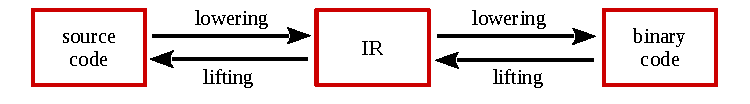
\includegraphics[width=.7\columnwidth]{images/compiler} 
\end{figure}


